\documentclass{article}

\usepackage{amsmath}
\usepackage{amsfonts} % For math fonts.
\usepackage{amssymb} % For other math symbols not covered by amsmath.
\usepackage[pdftex]{graphicx} % For pictures, use %\includegraphics[scale=decimal]{pic.png}; must be a .png file type.
\usepackage{multicol}
\usepackage{textcomp}
\usepackage[colorlinks = true, urlcolor = blue]{hyperref}
\usepackage{enumitem}
\usepackage{graphbox} 
\usepackage{subfig}
\usepackage{multicol}

\newcommand{\tab}{\hspace*{0.25in}}

\usepackage{tikz}
\usetikzlibrary{positioning, calc}
\usetikzlibrary{shapes.geometric,angles,quotes}
\usepackage{tikz-3dplot}

\newcommand{\csq}[1]{\reflectbox{''}#1''}  %This produces CS style quotes.



\usepackage{fullpage}
\usepackage{listings}
\lstset
{ %Formatting for code in appendix
    language=Python,
    basicstyle=\footnotesize,
    numbers=left,
    stepnumber=1,
    showstringspaces=false,
    tabsize=2,
    breaklines=true,
    breakatwhitespace=false,
}


\begin{document}


\begin{flushright}
functions\end{flushright}

\vspace*{-1.5em}
\noindent\makebox[\linewidth]{\rule{\paperwidth}{0.4pt}}


\vspace*{2em}

\begin{enumerate}


%standard 9.1
%week 8


%start_of_questions


%new_question
%%%%%%%%%%%%%%%%%%%%%
	% Problem 1
	% Difficulty: 1
%%%%%%%%%%%%%%%%%%%%%
	\item 
		(Game: heads or tails)  Write a \textbf{function} that lets the user guess whether the flip of a coin 
		results in heads or tails. The function randomly generates an integer 0 or 1, which 
		represents head or tail. The function returns if the guess is correct or incorrect. The argument for the function will be $guess$ 
		(the guess of the user, 0 for heads and 1 for tails), if no argument is provided then the \textbf{default} should be 0 for heads.\\
		Hint: Use the following lines of code to create the function.
		\begin{verbatim}
		    from random import randint
		    value = randint(0,1) #picks a random integer. Either 0 or 1.
		\end{verbatim}
		\textbf{Examples:}
		\begin{itemize}
			\item  toss\_coin( ) $\rightarrow$ \csq{Correct!} (if the random value is 0) or 
				\csq{Incorrect!} (if the random value is 1), 
			\item  toss\_coin(0) $\rightarrow$ \csq{Correct!} (if the random value is 0) or 
				\csq{Incorrect!} (if the random value is 1), 
			\item  toss\_coin(1) $\rightarrow$ \csq{Correct!} (if the random value is 1) or 
				\csq{Incorrect!} (if the random value is 0) 
		\end{itemize}

%new_question
%%%%%%%%%%%%%%%%%%%%%
	% Problem 2
	% Difficulty: 1
%%%%%%%%%%%%%%%%%%%%%
	\item 
		(Game: Odd or Even)  Write a \textbf{function} that lets the user guess whether a randomly 
		generated number is odd or even.  The function randomly generates an integer between 0 and 9 
		(inclusive) and returns whether the user's guess is correct or incorrect. The argument for 
		the function will be $guess$ (the user's guess, either \csq{odd} or \csq{even}), if no 
		argument is provided then the \textbf{default} guess should be even.\\
		Hint: Use the following lines of code to create the function.
		\begin{verbatim}
		    from random import randint
		    value = randint(0,9) #picks a random integer between 0-9 inclusive
		\end{verbatim}
		\textbf{Examples:}
		\begin{itemize}
			\item  guess( ) $\rightarrow$ \csq{Correct!} (if random value is even) 
				or \csq{Incorrect!} (if random value is odd) 
			\item  guess(\csq{odd})$\rightarrow$\csq{Correct!} (if random value is odd) 
				or \csq{Incorrect!} (if random value is even)
			\item  guess(\csq{even}) $\rightarrow$ \csq{Correct!} (if random value is even) 
				or \csq{Incorrect!} (if random value is odd) 
		\end{itemize}

%new_question
%%%%%%%%%%%%%%%%%%%%%
	% Problem 3
	% Difficulty: 1
%%%%%%%%%%%%%%%%%%%%%
	\item 
		Write a \textbf{function} that returns the number of copies of the same number. 
		The arguments for the function will be $num\_1$ (first number), $num\_2$ (second number), 
		and $num\_3$ (third number), if no argument is provided then the \textbf{default} for all 
		3 values should be 0.\\

		\textbf{Examples:}		
		\begin{itemize}
			\item  count\_duplicates(2, 3, 2) $\rightarrow$ \csq{There are 2 of the same number}, 
			\item  count\_duplicates(4, 4, 4) $\rightarrow$ \csq{There are 3 of the same number}, 
			\item  count\_duplicates(1, 2, 3) $\rightarrow$ \csq{Each number is unique} 
			\item  count\_duplicates(1) $\rightarrow$ \csq{There are 2 of the same number} 
			\item  count\_duplicates(0) $\rightarrow$ \csq{There are 3 of the same number} 
		\end{itemize}


%new_question
%%%%%%%%%%%%%%%%%%%%%
	% Problem 4
	% Difficulty: 1
%%%%%%%%%%%%%%%%%%%%%
	\item 
		Write a \textbf{function} to create a game of Rock, Paper, Scissors. The function will 
		return the winner of the game played by two players.
		The arguments to the function will be $player1$ (the first player's choice) and $player2$ 
		(the second player's choice), if no argument is provided then the \textbf{default} for 
		either player should be Rock.\\
		Print the winner according to the following rules. 
		\begin{itemize}
			\item Rock beats Scissors
			\item Scissors beats Paper
			\item Paper beats Rock
		\end{itemize}		
		\textbf{Examples:}		
		\begin{itemize}
			\item  find\_winner(\csq{Rock}, \csq{Paper}) $\rightarrow$ \csq{Player 2 wins!}, 
			\item  find\_winner(\csq{Scissors}, \csq{Paper}) $\rightarrow$ \csq{Player 1 wins!}, 
			\item  find\_winner(\csq{Rock}, \csq{Rock}) $\rightarrow$ \csq{It's a tie!}
			\item  find\_winner(\csq{Rock}) $\rightarrow$ \csq{It's a tie!}
			\item  find\_winner( ) $\rightarrow$ \csq{It's a tie!}
			\item  find\_winner(\csq{Scissors}) $\rightarrow$ \csq{Player 2 wins!}
		\end{itemize}


%new_question
%%%%%%%%%%%%%%%%%%%%%
	% Problem 5
	% Difficulty: 1
%%%%%%%%%%%%%%%%%%%%%
	\item 
		Luke Skywalker has friends and family, but he is getting older and having trouble 
		remembering them all.  Write a \textbf{function} that will return the relation 
		defined in the table below. The arguments to the function will be $name$ 
		(name of the person related to Luke), if no argument is provided then the 
		\textbf{default} should be nothing. That is, the empty word \csq{ }. \\ 
		\begin{center}
		\begin{tabular}{|l|l|} \hline
			Person 		& Relation \\ \hline \hline
			Darth Vader	& Father \\ \hline
			Leia		& Sister \\ \hline
			Han			& Brother in law\\ \hline
			R2D2		& Droid \\ \hline
		\end{tabular}\\ \hspace*{1in} *If he types any other name, return \csq{unknown}.
		\end{center}
		\textbf{Examples:}		
		\begin{itemize}
			\item  find\_relation(\csq{Darth Vader}) $\rightarrow$ \csq{Father}, 
			\item  find\_relation(\csq{R2D2}) $\rightarrow$ \csq{Droid}, 
			\item  find\_relation(\csq{Jabba the Hutt}) $\rightarrow$ \csq{Unknown}
			\item  find\_relation( ) $\rightarrow$ \csq{Unknown}
		\end{itemize}


%new_question
%%%%%%%%%%%%%%%%%%%%%
	% Problem 6
	% Difficulty: 1
%%%%%%%%%%%%%%%%%%%%%
	\item 
		Given a positive integer $n$, the following rules will always create a sequence that 
		ends with 1, called Hailstone Sequence:
		\begin{enumerate}
			\item If $n$ is even, divide by 2
			\item If $n$ is odd, multiply by 3 and add 1 (i.e. $3n+1$)
			\item Continue until $n$ is 1
		\end{enumerate}
		Write a \textbf{function} that prints the hailstone sequence starting at $n$. 
		The argument to the function will be $n$ (the integer to start the sequence from), 
		if no argument is provided then the \textbf{default} should be 40.
		\textbf{Examples:}		
		\begin{itemize}
			\item  hailstone\_seq(25) $\rightarrow$ 25, 76, 38, 19, 58 ... 8, 4, 2, 1, 
			\item  hailstone\_seq(40) $\rightarrow$ 40, 20, 10, 5, 16, 8, 4, 2, 1
			\item  hailstone\_seq( ) $\rightarrow$ 40, 20, 10, 5, 16, 8, 4, 2, 1
		\end{itemize}


%new_question
%%%%%%%%%%%%%%%%%%%%%
	% Problem 7
	% Difficulty: 1
%%%%%%%%%%%%%%%%%%%%%
	\item
		Write a \textbf{function} that takes 3 numbers as arguments, $num\_1$ (first number), 
		$num\_2$ (second number), and $num\_3$ (third number).  $num\_1$ should be mandatory.
		If no arguments are provided for $num\_2$ or $num\_3$ then use 5 for $num\_2$ and 
		25 for $num\_3$.
		Return a list of the integers in ascending order. \\
		You may \textbf{not} use the built-in functions \textit{max}(), \textit{min}(), 
		\textit{sort}(), or \textit{sorted}().
		
	\textbf{Examples:}
	\begin{itemize}
		\item  ascending\_order(2, 3, 1) $\rightarrow$ [1, 2, 3], 
		\item  ascending\_order(10, 1) $\rightarrow$ [1, 10, 25], 
		\item  ascending\_order(50) $\rightarrow$ [5, 25, 50] 
	\end{itemize}


%new_question
%%%%%%%%%%%%%%%%%%%%%
	% Problem 8
	% Difficulty: 1
%%%%%%%%%%%%%%%%%%%%%
	\item
		Write a \textbf{function} that takes 3 numbers as arguments, $num\_1$ (first number), 
		$num\_2$ (second number), and $num\_3$ (third number).  $num\_1$ should be mandatory.
		If no arguments are provided for $num\_2$ or $num\_3$ then use 15 for $num\_2$ and 
		5 for $num\_3$.
		Return a list of the integers in descending order. 
		You may \textbf{not} use the built-in functions \textit{max}(), \textit{min}(), 
		\textit{sort}(), or \textit{sorted}().
		
	\textbf{Examples:}
	\begin{itemize}
		\item  descending\_order(2, 3, 1) $\rightarrow$ [3, 2, 1], 
		\item  descending\_order(10) $\rightarrow$ [15, 10, 5], 
		\item  descending\_order(2, 45) $\rightarrow$ [45, 5, 2] 
	\end{itemize}


%new_question
%%%%%%%%%%%%%%%%%%%%%
	% Problem 9
	% Difficulty: 1
%%%%%%%%%%%%%%%%%%%%%
	\item
		Write a \textbf{function} that takes two arguments, a list and a value.  The function 
		should return the indices of all occurrences of the $value$ in the list, 
		if no argument is provided then the \textbf{default} should be to find 0.

		\textbf{Examples:}		
		\begin{itemize}
			\item  get\_indices( [1, 0, 5, 0, 7] ) $\rightarrow$ [1, 3]
			\item  get\_indices( [1, 5, 5, 2, 7], 7) $\rightarrow$ [4]
			\item  get\_indices( [1, 5, 5, 2, 7] ) $\rightarrow$ [ ]
			\item  get\_indices( [1, 5, 5, 2, 7], 5) $\rightarrow$ [1, 2]
			\item  get\_indices( [1, 5, 5, 2, 7], 8) $\rightarrow$ [ ]
			\item  get\_indices( [\csq{a}, \csq{a}, \csq{b}, \csq{a}, \csq{b}, \csq{a}], \csq{a}) 
				$\rightarrow$ [0, 1, 3, 5]
		\end{itemize}


%new_question
%%%%%%%%%%%%%%%%%%%%%
	% Problem 10
	% Difficulty: 1
%%%%%%%%%%%%%%%%%%%%%
	\item 
		Write a \textbf{function} that returns the factors of a given integer. 
		The argument of the function will be $num$ (integer to find factors for), 
		if no argument is provided then the \textbf{default} should be 36.

		\textbf{Examples:}		
		\begin{itemize}
			\item  find\_factors(12) $\rightarrow$ 1, 2, 3, 4, 6, 12, 
			\item  find\_factors(17) $\rightarrow$ 1, 17,
			\item  find\_factors(36) $\rightarrow$ 1, 2, 3, 4, 6, 9, 12, 18, 36
			\item  find\_factors( ) $\rightarrow$ 1, 2, 3, 4, 6, 9, 12, 18, 36
		\end{itemize}


%new_question
%%%%%%%%%%%%%%%%%%%%%
	% Problem 11
	% Difficulty: 1
%%%%%%%%%%%%%%%%%%%%%
	\item
		Write a \textbf{function} that takes two numbers as arguments $num$ and $length$ and 
		returns a list of multiples of $num$ until the list length reaches $length$, if no 
		argument is provided then the \textbf{default} for the list length should be 5.

		\textbf{Examples:}		
		\begin{itemize}
			\item  list\_of\_multiples(7, 5) $\rightarrow$ [7, 14, 21, 28, 35]
			\item  list\_of\_multiples(12, 10) $\rightarrow$ [12, 24, 36, 48, 60, 72, 84, 96, 108, 120]
			\item  list\_of\_multiples(2) $\rightarrow$ [2, 4, 6, 8, 10]
			\item  list\_of\_multiples(2,3) $\rightarrow$ [2, 4, 6]
		\end{itemize}




%end_of_questions
%make sure to leave at least one blank line below


%standard 9.2
%week 8


%start_of_questions



%new_question
%%%%%%%%%%%%%%%%%%%%%
	% Problem 12
	% Difficulty: 2
%%%%%%%%%%%%%%%%%%%%%
	\item 
		Write a \textbf{function} named \textit{is\_even} that returns a boolean value which determines 
		if an integer is even.  Write a second function named \textit{report\_evens} that takes a list 
		of integers and returns a new list containing all the even numbers from the original list. 
		Call the \textit{is\_even} function as part of the \textit{report\_evens} function. 
		
		\begin{itemize}
			\item  report\_evens([4,3,12,16,8,9,25]) $\rightarrow$ [4,12,16,8]
			\item  report\_evens([6,100,3,12,16,6,9,100]) $\rightarrow$ [6,100,12,16,6,100]
			\item  report\_evens([3,99,7,13,25]) $\rightarrow$ []
		\end{itemize}


%new_question
%%%%%%%%%%%%%%%%%%%%%
	% Problem 13
	% Difficulty: 2
%%%%%%%%%%%%%%%%%%%%%
	\item 
		Write a \textbf{function} named \textit{is\_vowel} that returns a boolean value which determines 
		if an letter is a vowel.  Write a second function named \textit{report\_vowels} that takes a string 
		and returns a list containing all the vowels from the original string.
		Call the \textit{is\_vowel} function as part of the \textit{report\_vowels} function. 

		Hint: In the English language, the letters a, e, i, o, and u are the vowels.\\
		\textbf{Examples:}		
		\begin{itemize}
			\item report\_vowels(\csq{apple}) $\rightarrow$ [a,e]
			\item report\_vowels(\csq{banana}) $\rightarrow$ [a,a,a] 
			\item report\_vowels(\csq{run time error}) $\rightarrow$ [r,i,e,e,o]
		\end{itemize}

	

%new_question
%%%%%%%%%%%%%%%%%%%%%
	% Problem 14
	% Difficulty: 2
%%%%%%%%%%%%%%%%%%%%%
	\item 
		Write a \textbf{function} named \textit{is\_two\_digit\_number} that returns a boolean value 
		which determines if an integer is a two digit number. Write a second function named 
		\textit{report\_two\_digit\_numbers} that takes a list of integers and returns a new list 
		containing all the two digit numbers from the original list. 
		Call the \textit{is\_two\_digit\_number} function as part of the \textit{report\_two\_digit\_numbers} function. 

		Hint: a two digit number is one in the range $[-99,-10]\cup[10,99]$.\\
		\textbf{Examples:}		
		\begin{itemize}
			\item report\_two\_digit\_numbers([100,57,12,1]) $\rightarrow$ [57,12]
			\item report\_two\_digit\_numbers([121,36,-19,-6,0,21]) $\rightarrow$ [36,-19,21]
			\item report\_two\_digit\_numbers([100,7,8437]) $\rightarrow$ []
		\end{itemize}



%new_question
%%%%%%%%%%%%%%%%%%%%%
	% Problem 15
	% Difficulty: 2
%%%%%%%%%%%%%%%%%%%%%
	\item 
		Write a function named \textit{is\_negative} that returns a boolean value which determines 
		if an integer is a negative number. 
		Write a second function named \textit{is\_odd} that returns a boolean value which determines 
		if an integer is odd.
		Write a third function named \textit{report\_negative\_odds} that takes a list of integers 
		and returns a new list containing all the negative odd numbers from the original list. 
		The \textit{report\_negative\_odds} function must call the \textit{is\_negative} and 
		\textit{is\_odd} to	determine if an element belongs.
		
		\textbf{Examples:}		
		\begin{itemize}
			\item report\_negative\_odds([100,-57,12,1,-36,-15]) $\rightarrow$ [-57,-15]
			\item report\_negative\_odds([121,-101,36,-19,-6,0,21,-1]) $\rightarrow$ [-101,-19,-1]
			\item report\_negative\_odds([-100,7,8437]) $\rightarrow$ []
		\end{itemize}




%end_of_questions
%make sure to leave at least one blank line below






\end{enumerate}
\end{document}




%\item Write a program that will convert some amount of pennies into the fewest amount of dollars and coins possible.  For example, 75 pennies is 3 quarters.  86 pennies is 3 quarters, 1 dime, and 1 penny.  130 pennies is 1 dollar, 1 quarter and 1 nickel.  Let the user pick the number of pennies.  You may assume the largest input is 499 pennies.\\
%Hint: the way to do this is to always substitute for the largest denomination if available.  For example, if there is at least 100 pennies substitute for a dollar before quarters.
















%new_question
%%%%%%%%%%%%%%%%%%%%%
	% Problem 1
	% Difficulty: 1
%%%%%%%%%%%%%%%%%%%%%
\item
	Write a \textbf{function} that takes a dictionary, called $employee\_salaries$, where the keys are employee names and the values are their salaries.
	The function should return a list of employees earning above a given salary. If no argument is provided then \textbf{default} to finding salaries above 65000.
	
	\textbf{Examples:}  
	\begin{itemize}  
		\item high\_earners(\{\csq{Alice}: 50000, \csq{Bob}: 75000, \csq{Charlie}: 100000\}, 60000) $\rightarrow$ [\csq{Bob}, \csq{Charlie}]
		\item high\_earners(\{\csq{David}: 30000, \csq{Emma}: 45000, \csq{Frank}: 50000\}, 40000) $\rightarrow$ [\csq{Emma}, \csq{Frank}]
		\item high\_earners(\{\csq{George}: 25000, \csq{Hannah}: 27000, \csq{Ian}: 29000\}, 30000) $\rightarrow$ []
	\end{itemize}





%new_question
%%%%%%%%%%%%%%%%%%%%%
	% Problem 1
	% Difficulty: 1
%%%%%%%%%%%%%%%%%%%%%
	\item 
		In Harry Potter, the currency consists of knuts, sickle, and galleon. There are 29 knuts in 
		one sickle and 17 sickles in one galleon. Write a \textbf{function} that will return a 
		converted amount of knuts into the fewest amount of coins possible. Only return a string 
		with the non-zero values, meaning don't return something similar to ``0 sickles''. The 
		argument for the function will be $knuts$ (how many knuts to convert), if no argument is provided then the \textbf{default} should be 900 knuts. 

		\textbf{Examples:}
		\begin{itemize}
			\item  convert\_knuts(32) $\rightarrow$ \csq{1 sickle 3 knuts}, 
			\item  convert\_knuts(544) $\rightarrow$ \csq{1 galleon 4 sickles 18 knuts}, 
			\item  convert\_knuts(993) $\rightarrow$ \csq{2 galleons 7 knuts}\\
				Note: Do \textbf{not} output 2 galleons 0 sickle 7 knuts.
		\end{itemize}



%new_question
%%%%%%%%%%%%%%%%%%%%%
	% Problem 1
	% Difficulty: 1
%%%%%%%%%%%%%%%%%%%%%
	\item 
		Detective Sherlock Holmes is solving cases, but he sometimes forgets the key suspects 
		in his investigations. Write a \textbf{function} that will return the suspect defined 
		in the table below. The arguments to the function will be $name$ (name of the suspect), 
		if no argument is provided then the \textbf{default} should be Mrs. Hudson.\\ 
		\begin{center}
		\begin{tabular}{|l|l|} \hline
			Person 		& Role \\ \hline \hline
			Moriarty	& Archenemy \\ \hline
			Watson		& Best Friend \\ \hline
			Mrs. Hudson			& Landlady \\ \hline
			Inspector Lestrade		& Detective \\ \hline
		\end{tabular}\\ \hspace*{1in} *If he types any other name, return \csq{unknown}.
		\end{center}
		\textbf{Examples:}		
		\begin{itemize}
			\item  find\_relation(\csq{Moriarty}) $\rightarrow$ \csq{Archenemy}, 
			\item  find\_relation(\csq{Mrs. Hudson}) $\rightarrow$ \csq{Landlady}, 
			\item  find\_relation(\csq{Mycroft Holmes}) $\rightarrow$ \csq{Unknown}
		\end{itemize}






%new_question
%%%%%%%%%%%%%%%%%%%%%
	% Problem 1
	% Difficulty: 1
%%%%%%%%%%%%%%%%%%%%%
	%new
		%https://edabit.com/challenge/aqDGJxTYCx7XWyPKc
	\item 

		Write a \textbf{function} that returns the sum of the squares of all positive integers up to a given integer (inclusive). The
		argument to the function will be $num$ (the number up to which squares should be summed).
 
		\textbf{Examples:}		
		\begin{itemize}
			\item  square\_sum(3) $\rightarrow$ 14 ($1^2 + 2^2 + 3^2 = 14$)
			\item  square\_sum(8) $\rightarrow$ 204 ($1^2+2^2+3^2+4^2+5^2+6^2+7^2+8^2=204$)
			\item  square\_sum(-3) $\rightarrow$ \csq{unknown}
		\end{itemize}


%new_question
%%%%%%%%%%%%%%%%%%%%%
	% Problem 1
	% Difficulty: 1
%%%%%%%%%%%%%%%%%%%%%
	%new
	\item 
		Write a \textbf{function} that returns the sum of the cubes of all positive integers up to a given integer (inclusive). The
		argument to the function will be $num$ (the number up to which cubes should be summed).

		\textbf{Examples:}		
		\begin{itemize}
			\item  cube\_sum(3) $\rightarrow$ 36 ($1^3 + 2^3 + 3^3 = 36$)
			\item  cube\_sum(8) $\rightarrow$ 1296 ($1^3+2^3+3^3+4^3+5^3+6^3+7^3+8^3=1296$)
			\item  cube\_sum(-3) $\rightarrow$ \csq{unknown}
		\end{itemize}



%new_question
%%%%%%%%%%%%%%%%%%%%%
	% Problem 1
	% Difficulty: 1
%%%%%%%%%%%%%%%%%%%%%
	\item 
		The table below show what your resting heart rate should be based on age and athleticism. 
		Write a \textbf{function} that returns what the resting heart rate of the user should be. 
		The arguments for the function will be $age$ (how old the user is) and $athl\_goal$ (athletic goal of user).
	\begin{center}
		\begin{minipage}{.45\textwidth}
			\begin{tabular}{c|cc}
				& \multicolumn{2}{c}{Athleticism}\\
				Age & Above Average & Below Average \\ \hline
				20 -- 39 & 47 -- 72 & 73 -- 93\\
				40 -- 59 & 46 -- 71 & 72 -- 94\\
				60 -- 79 & 45 -- 70 & 71 -- 97 \\
			\end{tabular}
		\end{minipage}
	\end{center}

	\textbf{Examples:}
	\begin{itemize}
		\item  resting\_rate(45, \csq{Below Average}) $\rightarrow$ \csq{72-94}, 
		\item  resting\_rate(79, \csq{Above Average}) $\rightarrow$ \csq{45-70}, 
		\item  resting\_rate(20, \csq{Below Average}) $\rightarrow$ \csq{73-93} 
	\end{itemize}


%new_question
%%%%%%%%%%%%%%%%%%%%%
	% Problem 1
	% Difficulty: 1
%%%%%%%%%%%%%%%%%%%%%
	\item 
		The table below shows what time different age groups (by grade) can swim at the pool.  There 
		are two time options, morning and afternoon.  Write a \textbf{function} that returns the time 
		the pool is available for the user. The arguments for the function will be $grade$ (which grade the user is in) 
		and $time$ (which time the user would like to go in).
	\begin{center}
		\begin{minipage}{.45\textwidth}
			\begin{tabular}{c|cc}
				& \multicolumn{2}{c}{Pool times}\\
				Grade 		& Morning 	& Afternoon \\ \hline
				k, 1 -- 3 	& 9 AM 		& 1 PM\\
				4 -- 8 		& 10 AM 	& 2 PM\\
				9 -- 12 	& 11 AM 	& 3 PM \\
			\end{tabular}
		\end{minipage}
	\end{center}

	\textbf{Examples:}
	\begin{itemize}
		\item  pool\_time('k', \csq{Morning}) $\rightarrow$ \csq{9 AM}, 
		\item  pool\_time(5, \csq{Afternoon}) $\rightarrow$ \csq{2 PM}, 
		\item  pool\_time(12, \csq{Morning}) $\rightarrow$ \csq{11 AM}
	\end{itemize}

%new_question
%%%%%%%%%%%%%%%%%%%%%
	% Problem 1
	% Difficulty: 1
%%%%%%%%%%%%%%%%%%%%%
	\item
		When driving in a car and approaching a traffic control light, \textit{green} means go, 
		\textit{yellow} means yield, and \textit{red} means stop. Write a \textbf{function} that returns the action 
		that should be taken by a driver. The argument for the function will be 
		$light\_color$ (the current color of the traffic control light).

	\textbf{Examples:}
	\begin{itemize}
		\item  traffic\_light(\csq{red}) $\rightarrow$ \csq{Stop}, 
		\item  traffic\_light(\csq{Green}) $\rightarrow$ \csq{Go}, 
		\item  traffic\_light(\csq{Yellow}) $\rightarrow$ \csq{Yield}
	\end{itemize}


%new_question
%%%%%%%%%%%%%%%%%%%%%
	% Problem 1
	% Difficulty: 1
%%%%%%%%%%%%%%%%%%%%%
	%new
	\item
		When using a security access system, different clearance levels are assigned to users. 
		In our system, \textit{admin} means full access, \textit{user} means limited access, 
		and \textit{guest} means view-only access. Write a function named \textbf{access\_rights} 
		that takes user\_role (a string) as an argument and returns the access rights of a user. 

	\textbf{Examples:}
	\begin{itemize}
		\item  access\_rights(\csq{user}) $\rightarrow$ \csq{limited}, 
		\item  access\_rights(\csq{guest}) $\rightarrow$ \csq{view}, 
		\item  access\_rights(\csq{admin}) $\rightarrow$ \csq{full}
	\end{itemize}


%new_question
%%%%%%%%%%%%%%%%%%%%%
	% Problem 1
	% Difficulty: 1
%%%%%%%%%%%%%%%%%%%%%
	\item 
		Primary U.S. interstate highways are numbered 1-99.  Odd numbers (like 5 or 95) go north/
		south, and evens (like 10 or 82) go east/west.  Auxiliary highways are numbered 100-999, and 
		service the primary highway indicated by the rightmost two digits.  Thus, I-405 services 
		I-5, and I-290 services I-90.
		
		Note: 200 is not a valid auxiliary highway because 00 is not a valid primary highway 
		number.\\
		
		Write a \textbf{function} that returns whether the highway runs north/south or east/west or is an invalid highway number. The argument for the function 
		will be $highway\_num$(highway number provided).
		\textbf{Examples:}		
		\begin{itemize}
			\item  highway\_directions(5) $\rightarrow$ \csq{I-5 runs north/south}, 
			\item  highway\_directions(82) $\rightarrow$ \csq{I-82 runs east/west}, 
			\item  highway\_directions(200) $\rightarrow$ \csq{I-200 is an invalid highway number} 
		\end{itemize}





%new_question
%%%%%%%%%%%%%%%%%%%%%
	% Problem 1
	% Difficulty: 1
%%%%%%%%%%%%%%%%%%%%%
	\item 
		At the local ice cream store they have 3 flavors, which are Vanilla, Chocolate, and Strawberry.  
		Write a \textbf{function} that returns the selected flavor. If the chosen flavor is not available, let them know.
		The argument to the function will be $selected\_flavor$ (the user's selected flavor).\\
		\textbf{Examples:}		
		\begin{itemize}
			\item  serve\_icecream(\csq{Vanilla}) $\rightarrow$ \csq{Here is your vanilla ice cream!}, 
			\item  serve\_icecream(\csq{Mint}) $\rightarrow$ \csq{Sorry, we don't have mint ice cream.}, 
			\item  serve\_icecream(\csq{Chocolate}) $\rightarrow$ \csq{Here is your chocolate ice cream!} 
		\end{itemize}


%new_question
%%%%%%%%%%%%%%%%%%%%%
	% Problem 1
	% Difficulty: 1
%%%%%%%%%%%%%%%%%%%%%
	%new
	\item 
		At the local coffee shop they have 3 types of coffee, which are Espresso, Latte, and Cappuccino.  
		Write a \textbf{function} that returns the selected coffee type. If the chosen type is not available, let them know.
		The argument to the function will be $selected\_coffee$ (the user's selected coffee type).\\
		\textbf{Examples:}		
		\begin{itemize}
			\item  serve\_coffee(\csq{Latte}) $\rightarrow$ \csq{Here is your latte!}, 
			\item  serve\_coffee(\csq{Mocha}) $\rightarrow$ \csq{Sorry, we don't have mocha.}, 
			\item  serve\_coffee(\csq{Espresso}) $\rightarrow$ \csq{Here is your espresso!}
		\end{itemize}


%new_question
%%%%%%%%%%%%%%%%%%%%%
	% Problem 1
	% Difficulty: 1
%%%%%%%%%%%%%%%%%%%%%
	\item 
		%https://edabit.com/challenge/ancAxGEF9MsLWXDqe
		Write a \textbf{function} that returns if a triangle is a scalene, isosceles, or an equilateral. The arguments to the function will be 
		$side\_1$ (first side of the triangle), $side\_2$ (second side of the triangle), and $side\_3$ (third side of the triangle).\\
		The types of triangles are: 
		\begin{itemize}
			\item No sides equal: \csq{scalene}
			\item Two sides equal: \csq{isosceles}
			\item All sides equal: \csq{equilateral}	
		\end{itemize}
		\textbf{Examples:}		
		\begin{itemize}
			\item  triangle\_type(1, 2, 3) $\rightarrow$ \csq{scalene}, 
			\item  triangle\_type(4, 4, 4) $\rightarrow$ \csq{equilateral}, 
			\item  triangle\_type(7, 7, 3) $\rightarrow$ \csq{isosceles} 
		\end{itemize}








--------------------------------------------------------------------------------------------------------------------------------------

%new_question
%%%%%%%%%%%%%%%%%%%%%
	% Problem 1
	% Difficulty: 1
%%%%%%%%%%%%%%%%%%%%%
	\item 
		%https://edabit.com/challenge/Ay9wPrqRJnBmvbFmi
		Ask the user for two integers, \textit{larger} and \textit{smaller}.  Determine (and output) 
		how many times larger can be halved while still be greater than smaller.
		
		Examples:
		\begin{itemize}
			\item if \textit{larger} = 1324 and  \textit{smaller} = 98, the result should be 3 since
				1324 $\rightarrow$ 662 $\rightarrow$ 331 $\rightarrow$ 165.5
			\item if \textit{larger} = 624 and  \textit{smaller} = 8, the result should be 6 since\\
				\tab 624 $\rightarrow$ 312 $\rightarrow$ 156 $\rightarrow$ 78 $\rightarrow$ 39 
				$\rightarrow$ 19.5 $\rightarrow$ 9.75)
		\end{itemize}



%new_question
%%%%%%%%%%%%%%%%%%%%%
	% Problem 1
	% Difficulty: 1
%%%%%%%%%%%%%%%%%%%%%
	\item 
		%https://edabit.com/challenge/68KgdtdwabrXydZFM
		Create a function that takes an integer named \textit{number} 
		%and a character named \textit{gender} (\csq{m} for male, \csq{f} for female), 
		and returns the name of an ancestor or\\ descendant based on the table below.
		Your code should work for any integer.
		\begin{flushright}
	    	\begin{tabular}{|c|c|c|} \hline
				\textbf{Generation} &  \\ \hline
	    	    -3 	& great grandparent \\
	    	    -2 	& grandparent \\
	    	    -1 	& parent\\
	    	   	0 	& me! \\
	    	 	1 	& child \\
	    	 	2 	& grandchild \\
		   	  	3 	& great grandchild\\ 
		   	  	\vdots & \\
		   	  	6 & great great great great grandchild \\ \hline
		    \end{tabular}
		\end{flushright}



%new_question
%%%%%%%%%%%%%%%%%%%%%
	% Problem 1
	% Difficulty: 1
%%%%%%%%%%%%%%%%%%%%%
	\item
		Write a \textbf{function} that calculates and returns the volume of a sphere.  
		The function should have the radius as an argument.
		Use the value of $\pi$ from the math module in your calculation.\\	
		Hint: $V = \dfrac{4}{3}\pi r^3 $

\begin{tabular}{l c}
	\begin{minipage}{0.5\textwidth}
		Examples:
		\begin{itemize}
			\item sphere\_volume(1) $\rightarrow$ 4.18, 
			\item sphere\_volume(0.9) $\rightarrow$ 3.05, 
			\item sphere\_volume(3) $\rightarrow$ 113.09, 
		\end{itemize}
	\end{minipage}

	\begin{minipage}{0.4\textwidth}
		\begin{flushright}
			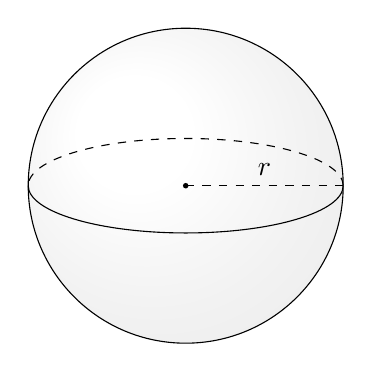
\begin{tikzpicture}
			\shade[ball color = white, opacity = 0.1] (0,0) circle (2cm);
			\draw (0,0) circle (2cm);
			\draw (-2,0) arc (180:360:2 and 0.6);
			\draw[dashed] (2,0) arc (0:180:2 and 0.6);
			\fill[fill=black] (0,0) circle (1pt);
			\draw[dashed] (0,0 ) -- node[above]{$r$} (2,0);
			\end{tikzpicture}
		\end{flushright}
\end{minipage}
\end{tabular}

%new_question
%%%%%%%%%%%%%%%%%%%%%
	% Problem 1
	% Difficulty: 1
%%%%%%%%%%%%%%%%%%%%%
	\item
		Write a \textbf{function} that calculates and then returns the area of a semi--circle.  	
		The function should have the radius as an argument.
		Use the value of $\pi$ from the math module in your calculation.\\	
		Hint: $A = \dfrac{1}{2}\pi r^2 $

\begin{tabular}{l c}
	\begin{minipage}{0.5\textwidth}
		Examples:
		\begin{itemize}
			\item semicircle\_area(0.8) $\rightarrow$ 1.00, 
			\item semicircle\_area(2) $\rightarrow$ 6.28, 
			\item semicircle\_area(5) $\rightarrow$ 39.26, 
		\end{itemize}
	\end{minipage}

	\begin{minipage}{0.4\textwidth}
		\begin{flushright}
			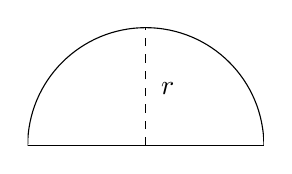
\begin{tikzpicture}[baseline=(current bounding box.north)]
				\begin{scope}
		    		\clip (-1.5,0) rectangle (1.5,1.5);
		    		\draw (0,0) circle(1.5);
					\draw (-1.5,0) -- (1.5,0);
					\draw[dashed] (0,0) -- (0,2);
				\end{scope}
				\node[below right= 1mm of {(0,1)}] {$r$};
			\end{tikzpicture}
		\end{flushright}
\end{minipage}
\end{tabular}

%maybe
%https://edabit.com/challenge/eADRy5SA5QbasA3Qt



%new_question
%%%%%%%%%%%%%%%%%%%%%
	% Problem 1
	% Difficulty: 1
%%%%%%%%%%%%%%%%%%%%%
	\item 
		Write a function that takes 3 numbers as arguments, $num\_1$ (first number), $num\_2$ (second number), and $num\_3$ (third number).  Return a list of the integers in ascending order. 
		You may \textbf{not} use the built-in functions \textit{max}(), \textit{min}(), \textit{sort}(), or \textit{sorted}().
		
	\textbf{Examples:}
	\begin{itemize}
		\item  ascending\_order(2, 3, 1) $\rightarrow$ [1, 2, 3], 
		\item  ascending\_order(10, 1, 25) $\rightarrow$ [1, 10, 25], 
		\item  ascending\_order(2, 45, 4) $\rightarrow$ [2, 4, 45] 
	\end{itemize}

		Write a \textbf{function} that returns three integers in increasing order (smallest to largest). 
		The arguments for the function will be $num\_1$ (first number), $num\_2$ (second number), 
		and $num\_3$ (third number).\\  
		You may \textbf{not} use the built-in functions \textit{max}(), \textit{min}(), \textit{sort}(), or \textit{sorted}().

	\textbf{Examples:}
	\begin{itemize}
		\item  ascending\_order(2, 3, 1) $\rightarrow$ 1, 2, 3, 
		\item  ascending\_order(10, 1, 25) $\rightarrow$ 1, 10, 25, 
		\item  ascending\_order(2, 45, 4) $\rightarrow$ 2, 4, 45 
	\end{itemize}


%new_question
%%%%%%%%%%%%%%%%%%%%%
	% Problem 1
	% Difficulty: 1
%%%%%%%%%%%%%%%%%%%%%
	\item 
		Write a \textbf{function} that returns three integers in decreasing order (largest to smallest). 
		The arguments for the function will be $num\_1$ (first number), $num\_2$ (second number), 
		and $num\_3$ (third number).\\  
		You may \textbf{not} use the built-in functions \textit{max}(), \textit{min}(), \textit{sort}(), or \textit{sorted}().

	\textbf{Examples:}
	\begin{itemize}
		\item  descending\_order(2, 3, 1) $\rightarrow$ 3, 2, 1, 
		\item  descending\_order(10, 1, 25) $\rightarrow$ 25, 10, 1, 
		\item  descending\_order(2, 45, 4) $\rightarrow$ 45, 4, 2 
	\end{itemize}




%new_question
%%%%%%%%%%%%%%%%%%%%%
	% Problem 1
	% Difficulty: 1
%%%%%%%%%%%%%%%%%%%%%
	%new
	\item 
		Write a \textbf{function} that checks whether a letter has a descender or not.  The function should return \csq{Descender} if 
		the letter extends below the baseline and \csq{No Descender} otherwise. The argument to the function 
		will be $letter$ (a single lowercase letter).\\
		Hint: In the English language, the letters g, j, p, q, and y have descenders.\\
		\textbf{Examples:}		
		\begin{itemize}
			\item  check\_letter('g') $\rightarrow$ \csq{Descender}, 
			\item  check\_letter('z') $\rightarrow$ \csq{No Descender}, 
			\item  check\_letter('p') $\rightarrow$ \csq{Descender} 
		\end{itemize}


%new_question
%%%%%%%%%%%%%%%%%%%%%
	% Problem 1
	% Difficulty: 1
%%%%%%%%%%%%%%%%%%%%%
	\item 
		%https://edabit.com/challenge/Ay9wPrqRJnBmvbFmi
		Write a \textbf{function} that will return how many times a larger integer can be halved
		while still remaining greater than a smaller integer. The arguments to the function will 
		be $larger$ (the larger number to be halved) and $smaller$ (the smaller number the halved
		 value must remain greater than).\\ 
		
		\textbf{Examples:}		
		\begin{itemize}
			\item if \textit{larger} = 1324 and  \textit{smaller} = 98, the result should be 3 since
				1324 $\rightarrow$ 662 $\rightarrow$ 331 $\rightarrow$ 165.5
			\item if \textit{larger} = 624 and  \textit{smaller} = 8, the result should be 6 since:\\
				\tab 624 $\rightarrow$ 312 $\rightarrow$ 156 $\rightarrow$ 78 $\rightarrow$ 39 
				$\rightarrow$ 19.5 $\rightarrow$ 9.75
		\end{itemize}

%new_question
%%%%%%%%%%%%%%%%%%%%%
	% Problem 1
	% Difficulty: 1
%%%%%%%%%%%%%%%%%%%%%
	%new
	\item 
		Write a \textbf{function} that will return how many times a smaller integer can be 
		doubled while still remaining less than a larger integer. The arguments to the function 
		will be $larger$ (the larger number the doubled value must remain less than) and 
		$smaller$ (the smaller number to be doubled).\\ 
		
		\textbf{Examples:}		
		\begin{itemize}
			\item if \textit{larger} = 1324 and  \textit{smaller} = 98, the result should be 3 since
				98 $\rightarrow$ 196 $\rightarrow$ 392 $\rightarrow$ 784
			\item if \textit{larger} = 624 and  \textit{smaller} = 8, the result should be 6 since:\\
				\tab 8 $\rightarrow$ 16 $\rightarrow$ 32 $\rightarrow$ 64 $\rightarrow$ 128 
				$\rightarrow$ 256 $\rightarrow$ 512
		\end{itemize}
		







%new_question
%%%%%%%%%%%%%%%%%%%%%
	% Problem 1
	% Difficulty: 1
%%%%%%%%%%%%%%%%%%%%%
	\item 
		In an Ancient Kingdom, the currency consists of bronze coins, silver coins, and gold coins.  
		There are 20 bronze coins in one silver coin and 15 silver coins in one gold coin.  Write a 	
		\textbf{function} that will return a converted amount of bronze coins into the fewest amount 
		of coins possible.  Only return a string with the non-zero values, meaning don't return 
		something similar to ``0 silver coins''. The argument for the function will be 
		$bronze\_coins$ (how many bronze coins to convert)., if no argument is provided then the 
		\textbf{default} should be 900 bronze coins 

		\textbf{Examples:}
		\begin{itemize}
			\item  convert\_bronze(32) $\rightarrow$ \csq{1 silver 12 bronze}, 
			\item  convert\_bronze(544) $\rightarrow$ \csq{1 gold 4 silver 4 bronze}, 
			\item  convert\_bronze(903) $\rightarrow$ \csq{3 gold 3 bronze}\\
				Note: Do \textbf{not} output 3 gold 0 silver 3 bronze.
			\item  convert\_bronze() $\rightarrow$ \csq{3 gold}\\
				Note: Do \textbf{not} output 3 gold 0 silver 0 bronze.
		\end{itemize}
